 % LuaLaTeX文書; 文字コーAドはUTF-8
 \documentclass[unicode,12pt, a4paper]{ltjsarticle}% 'unicode'が必要
 %\usepackage{luatexja}% 日本語したい
 \usepackage{luatexja-fontspec}
 %\usepackage[hiragino-pron]{luatexja-preset}% IPAexフォントしたい(ipaex)
 \usepackage[hiragino-pron,deluxe,expert,bold]{luatexja-preset}

 \usepackage[english]{babel}%多言語文書を作成する
 \usepackage{amsmath,amssymb}%標準数式表現を拡大する
 \usepackage{physics}
 \usepackage{tikz}
 \usetikzlibrary{math}
 \usepackage{caption}
 \usepackage{subcaption}
 \usepackage[subpreambles=true,sort=true]{standalone}
% \renewcommand{\kanjifamilydefault}{\gtdefault}% 既定をゴシック体に
 \usepackage[backend=bibtex,style=phys,articletitle=false,biblabel=brackets,chaptertitle=false,pageranges=false]{biblatex}
 %\usepackage[style=authoryear,backend=bibtex]{biblatex}


 %\addbibresource{../references/tio2_ref.bib}
 \usepackage{mhchem}
 % あとは欧文の場合と同じ

  \usepackage{caption}
  \usepackage[subrefformat=parens]{subcaption}
\title{東工大理系後期1998年度}

\begin{document}
\maketitle
\section{問題1}
極限値 $\displaystyle \lim_{n \to \infty} \int_0^\frac{\pi}{2} \frac{\sin^2 nx}{1+x} dx$ を求めよ.



\section{問題2}
\begin{enumerate}
    \item 半径 $1$ の円に内接する $6$ 個の半径の等しい円を図 $1$ のように描き,さらに図 $2$ のように $6$ 個の小さな半径の等しい円を描く,この操作を無限にくり返したとき,$6$ 個ずつ次々に描かれる円の面積の総和 $S_2$ と,それらの円の円周の長さの総和 $C_2$ を求めよ.
    \item (1) で $6$ 個の円を次々に描いていった.一般に,自然数 $n \ge 2$ に対して $3n$ 個の円を用いて同様の操作を行うとき,描かれる円の面積の総和 $S_n$ と,それらの円の円周の長さの総和 $C_n$ を求めよ.
    \item 数列 $S_2, S_3, S_4, \cdots$ の極限値を求めよ.
\end{enumerate}

\begin{figure}
  \centering
  \begin{subcaptionblock}{0.5\linewidth}
    \centering
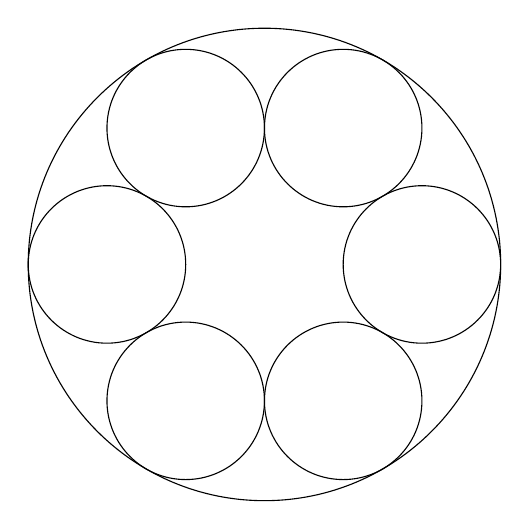
\begin{tikzpicture}
    % 中心に配置する円(オプション: 問題文には明示されていないが、図1には中心に円がない)
    % \draw (0,0) circle (0.5cm);

    % 周囲の6つの円
    % 外側の円の半径をR=3cmとする。
    % 周囲の円の半径をrとする。
    % 中心から周囲の円の中心までの距離をdとする。
    % d = R - r
    % また、中心から周囲の円の中心までの距離がd、周囲の円の半径がrであるとき、
    % sin(30度) = r / d より、d = 2r
    % よって、R - r = 2r => R = 3r => r = R/3
    % d = 2R/3
    \def\R{3} % 外側の円の半径
    \tikzmath{
    \r = \R / 3; % 周囲の円の半径
    \d = \R - \r; % 中心から周囲の円の中心までの距離
    }
    % 外側の大きな円
    \draw (0,0) circle (\R); % 適当なサイズに調整
    \foreach \i in {0, 60, ..., 300} {
        \draw ({\d*cos(\i)}, {\d*sin(\i)}) circle (\r cm);
    }
\end{tikzpicture}
\subcaption{図1}
\end{subcaptionblock}\hfill
  \begin{subcaptionblock}{0.5\linewidth}
    \centering
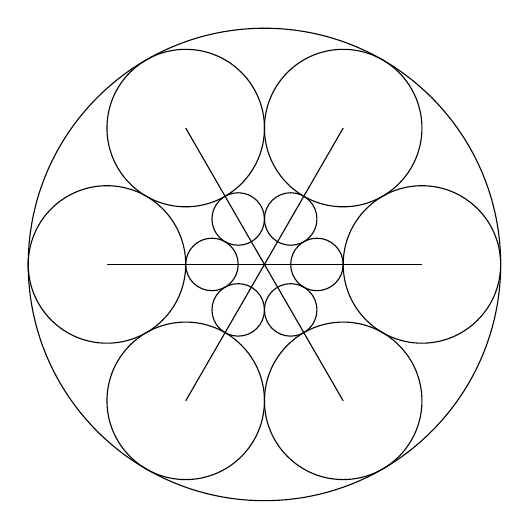
\begin{tikzpicture}
    \def\R{3} % 外側の円の半径
    \tikzmath{
    \r = \R / 3; % 周囲の円の半径
    \d = \R - \r; % 中心から周囲の円の中心までの距離
    }
    % 最も外側の大きな円(半径1と仮定)
    \draw (0,0) circle (\R);
    % 外側の大きな円
    \foreach \i in {0, 60, ..., 300} {
      \coordinate (C\i) at ({\d*cos(\i)}, {\d*sin(\i)});
      \draw (C\i) circle (\r);
      \draw (0,0) -- (C\i); % 中心から外側の円の中心への直線
    }
    \tikzmath{
    \rsmall = \r / 3; % 周囲の円の半径
    \dsmall = \r - \rsmall; % 中心から周囲の円の中心までの距離
    }
    % 内側の小きな円
    \foreach \i in {0, 60, ..., 300} {
        \draw ({\dsmall*cos(\i)}, {\dsmall*sin(\i)}) circle (\rsmall);
    }
\end{tikzpicture}
\subcaption{図2}
\end{subcaptionblock}\hfill
\end{figure}

\end{document}